%% This is file `sample-sigconf-authordraft.tex',
%% generated with the docstrip utility.
%%
%% The original source files were:
%%
%% samples.dtx  (with options: `all,proceedings,bibtex,authordraft')
%% 
%% IMPORTANT NOTICE:
%% 
%% For the copyright see the source file.
%% 
%% Any modified versions of this file must be renamed
%% with new filenames distinct from sample-sigconf-authordraft.tex.
%% 
%% For distribution of the original source see the terms
%% for copying and modification in the file samples.dtx.
%% 
%% This generated file may be distributed as long as the
%% original source files, as listed above, are part of the
%% same distribution. (The sources need not necessarily be
%% in the same archive or directory.)
%%
%%
%% Commands for TeXCount
%TC:macro \cite [option:text,text]
%TC:macro \citep [option:text,text]
%TC:macro \citet [option:text,text]
%TC:envir table 0 1
%TC:envir table* 0 1
%TC:envir tabular [ignore] word
%TC:envir displaymath 0 word
%TC:envir math 0 word
%TC:envir comment 0 0
%%
%%
%% The first command in your LaTeX source must be the \documentclass
%% command.
%%
%% For submission and review of your manuscript please change the
%% command to \documentclass[manuscript, screen, review]{acmart}.
%%
%% When submitting camera ready or to TAPS, please change the command
%% to \documentclass[sigconf]{acmart} or whichever template is required
%% for your publication.
%%
%%
%\documentclass[manuscript, screen, review]{acmart}
\documentclass[sigconf,authordraft]{acmart}

%%
%% \BibTeX command to typeset BibTeX logo in the docs
\AtBeginDocument{%
  \providecommand\BibTeX{{%
    Bib\TeX}}}

%% Rights management information.  This information is sent to you
%% when you complete the rights form.  These commands have SAMPLE
%% values in them; it is your responsibility as an author to replace
%% the commands and values with those provided to you when you
%% complete the rights form.
\setcopyright{acmlicensed}
\copyrightyear{2024}
\acmYear{2024}
\acmDOI{XXXXXXX.XXXXXXX}

%% These commands are for a PROCEEDINGS abstract or paper.
%\acmConference[Conference acronym 'XX]{Make sure to enter the correct conference title from your rights confirmation emai}{June 03--05, 2018}{Woodstock, NY}
%%
%%  Uncomment \acmBooktitle if the title of the proceedings is different
%%  from ``Proceedings of ...''!
%%
%%\acmBooktitle{Woodstock '18: ACM Symposium on Neural Gaze Detection,
%%  June 03--05, 2018, Woodstock, NY}
\acmISBN{978-1-4503-XXXX-X/18/06}
%%
%% Submission ID.
%% Use this when submitting an article to a sponsored event. You'll
%% receive a unique submission ID from the organizers
%% of the event, and this ID should be used as the parameter to this command.
%%\acmSubmissionID{123-A56-BU3}

%%
%% For managing citations, it is recommended to use bibliography
%% files in BibTeX format.
%%
%% You can then either use BibTeX with the ACM-Reference-Format style,
%% or BibLaTeX with the acmnumeric or acmauthoryear sytles, that include
%% support for advanced citation of software artefact from the
%% biblatex-software package, also separately available on CTAN.
%%
%% Look at the sample-*-biblatex.tex files for templates showcasing
%% the biblatex styles.
%%

%%
%% The majority of ACM publications use numbered citations and
%% references.  The command \citestyle{authoryear} switches to the
%% "author year" style.
%%
%% If you are preparing content for an event
%% sponsored by ACM SIGGRAPH, you must use the "author year" style of
%% citations and references.
%% Uncommenting
%% the next command will enable that style.
%%\citestyle{acmauthoryear}

\title{Towards Greener Networks: RApp-Based Cell Control Over O-RAN Deployments}
\author{Anonymous Authors}

%%
%% end of the preamble, start of the body of the document source.
\begin{document}

%%
%% The "title" command has an optional parameter,
%% allowing the author to define a "short title" to be used in page headers.

% ABSTRACT
\begin{abstract}

    Mobile communication technologies, in their quest to deliver the highest possible data rates over the air interface, have nearly touched the Shannon limit. 
    Despite the advancements in techniques to enhance service capabilities, the power usage by the radio and compute components at the base stations (known as eNodeB in LTE and gNodeB in NR) frequently constitutes a significant part of the operational costs (OPEX) for operators, a factor that is commonly disregarded.
    This paper delves into one of the most straightforward strategies for energy conservation in cellular networks: deactivating under-utilized cells.
    While there has been extensive research in this field, we present a novel, statistics-driven, and machine learning-assisted Energy Saving (ES) solution for Radio Access Network (RAN) cell shutdown.
    In addition, we introduce a novel validation framework for evaluating decision-making effectiveness and ensuring the Quality of Service (QoS) is maintained for end users.
    Our simulations, conducted over a O-RAN compliant rApp setup, demonstrate the effectiveness of the proposed technique, resulting in a significant reduction in power consumption.
    
\end{abstract}


\pagestyle{plain}
\maketitle

\section{Introduction}
\label{sec:intro}

%% WHAT IS THE PROBLEM?

With the advancements in techniques to pack maximum data over the communication channel, the Information and Communication Technology (ICT) industry has devised technologies which help us reach the Shannon’s limit on amount of data that can be reliably transferred over a channel. 
%This includes the use of efficient channel coding techniques, such as Low Density Parity Checks (LDPC), and the spatial reuse of channels, as seen in Multi-user MIMO. 
%The latter is often coupled with beamforming to direct data towards specific users or groups of users.
One of the most common methods to meet the ever-increasing service demands of the online public is harvesting more spectra for mobile communication networks, like the C-band which provides hundreds of MHz of bandwidth and millimeter wavelength spectrum which offers GHz of spectrum. 
%Achieving energy-efficiency in cellular networks is not practicable without paying special attention to the all energy consuming aspects of the network.
What is often overlooked are the aspects of practical realization of these techniques which demand huge computation resources both at the radio units as well as for processing within the base-band. 
The energy consumption of mobile networks is a significant concern, with the ICT industry accounting for 10\% of of the worldwide electricity consumption, a figure that is expected to double by 2025 \cite{ict-energy}.
Achieving energy efficiency in mobile networks, especially with the increasing deployment of 5G networks, is a significant issue facing the ICT industry to meet their goal of net zero emissions by 2050. 

Within a mobile network, Radio Access Networks (RAN) have been found to be one the most significant users of a mobile network's total power supplied\cite{ict1, ict2}.
% Recent advancements, such as the Open RAN (O-RAN) initiative \cite{oran}, have paved the way for the use of RAN Intelligent Controllers (RICs). 
% These flexible platforms provide robust control over RAN, and we have incorporated them into our system.
% The disaggregation introduced in O-RAN paves way for the introduction of several network optimization techniques without disturbing  core functionalities.
% O-RAN control is enabled using applications called xApps (for the Near-Real-Time RIC) and rApps (for the Non-Real-Time RIC), with the choice of the implementation made depending on the time-frame of the control required.

This paper examines one of the simplest techniques for energy savings - powering off unused nodes. 
It aims to establish formalisms for analyzing this technique and its impact on the Quality of Service (QoS) as perceived by the end users.
With the flexibility of implementation intrroduced by the O-RAN initiative, we have tested out the algorithim in a rApp compatible with any O-RAN compliant network. 
Our approach distinguishes itself from existing solutions by leveraging a statistically motivated framework rather than relying heavily on heuristics \cite{heuristics1,heuristics2}. 

Statistical approaches offer a more robust and data-driven foundation for decision-making compared to heuristic methods as is argued well in \cite{svh}. 
This approach allows for better adaptation to dependence on the inherent variability and unpredictability of network traffic patterns. 
%By utilizing statistical models, our solution can account for both short-term fluctuations and long-term trends in network usage, leading to more accurate and reliable cell shutdown decisions. 
%Moreover, statistical methods provide quantifiable measures of uncertainty and confidence, enabling network operators to make risk-aware decisions and better understand the potential impacts of their actions.
While previous implementations often employ techniques such as toggling between MIMO and SISO \cite{mimo-siso}, using reinforcement learning \cite{rl}, or realloacting BBUs \cite{bbu}, our method focuses on a more fundamental statistical analysis of network behavior. 
This statistical foundation allows for a more robust and generalizable solution that can be easily adapted to various network configurations without the need for extensive training or parameter tuning.
Unlike approaches that require specific network configurations or rely on proprietary systems, our method integrates seamlessly with the O-RAN architecture through the use of rApps. 
\hyperref[fig:system-architecture]{Figure 1} describes this interfacing with respect to traditional O-RAN architecture. 

By combining statistical rigor with O-RAN compatibility, our approach offers a unique balance of effectiveness and practicality that sets it apart from the more heuristic-driven or computationally intensive methods prevalent in the current literature.
The main contributions of this paper can be summarised as follows:
\begin{itemize}
    \item Introduced a statistical metric to evaluate the effectiveness of implemented policies, offering a method to validate decisions prior to implementation.
    \item Developed a swift and efficient method for cell shutdown, eliminating the need for excessive KPI calls or extensive training time.
    \item Implemented and detailed a novel solution that is readily deployable across all O-RAN compliant networks.
\end{itemize}

The remainder of this paper is organized into six sections, as follows.
Section 2 provides an overview of the problem at hand and outlines our proposed approach to address it.
Section 3 details our energy saving solution, while Section 4 provides an algorithm to arrive at an optimal solution.
The results obtained from the rApp evaluation using the software-defined NS-3 simulator are depicted and discussed in Section 5. 
Finally, Section 6 concludes the paper and suggests future research directions.

\definecolor{mygrey}{RGB}{145,146,156}
\definecolor{mypurple}{RGB}{153,102,204}
\definecolor{myotherblue}{RGB}{0,191,255}
\definecolor{mygreen}{RGB}{144,238,144}
\definecolor{myyellow}{RGB}{255,215,0}
\definecolor{myorange}{RGB}{255,165,0}
\definecolor{myothergreen}{RGB}{35,79,30}
\definecolor{myred}{RGB}{255,127,80}
\definecolor{myindigo}{RGB}{100,110,230}

\begin{figure}
    \centering
    \begin{tikzpicture}[
        subox1/.style={draw, fill=myorange, minimum width=1.1cm, minimum height=0.7cm, font=\footnotesize},
        subox2/.style={draw, fill=myindigo, minimum width=0.55cm, minimum height=0.7cm, font=\footnotesize},
        subox3/.style={draw, fill=myred, minimum width=0.55cm, minimum height=0.7cm, font=\footnotesize},
        subox4/.style={draw, fill=myothergreen, minimum width=2.4cm, minimum height=0.4cm, font=\footnotesize},
        box1/.style={draw, fill=mygreen, minimum width=2.6cm, minimum height=1.5cm, font=\footnotesize},
        box2/.style={draw, fill=myyellow, minimum width=1.7cm, minimum height=1.5cm, font=\footnotesize},
        smallbox1/.style={draw, fill=mypurple, minimum width=0.85cm, minimum height=0.5cm, font=\footnotesize, rounded corners},
        smallbox2/.style={draw, fill=myotherblue, minimum width=0.85cm, minimum height=0.5cm, font=\footnotesize, rounded corners},
        smallbox3/.style={draw, fill=mygrey, minimum width=0.85cm, minimum height=0.5cm, font=\footnotesize, rounded corners},
        flatbox1/.style={draw, fill=myotherblue, minimum width=2cm, minimum height=0.25cm, font=\footnotesize},
        flatbox2/.style={draw, fill=myotherblue, minimum width=3.2cm, minimum height=0.25cm, font=\footnotesize},
        flatbox3/.style={draw, fill=mygrey, minimum width=3.2cm, minimum height=0.35cm, font=\footnotesize},
        bigbox1/.style={draw, fill=myotherblue, minimum width=0.8cm, minimum height=0.7cm, font=\footnotesize},
        bigbox2/.style={draw, fill=mygrey, minimum width=0.75cm, minimum height=0.7cm, font=\footnotesize},
        bigbox3/.style={draw, fill=mygrey, minimum width=4.45cm, minimum height=0.4cm, font=\footnotesize},
        hugebox/.style={draw, , fill=mygrey, minimum width=9cm, minimum height=0.75cm, font=\footnotesize},
        scale=0.4 % Adjust this value to fit in one or two columns
    ]
    
    % Base layer
    \node[hugebox, text=white] (ns3) {\textbf{\texttt{ns-3 (network simulator)}}};

    % Second layer
    \node[smallbox1, text=white, above left=0.2 and -1.5 of ns3] (sdnr) {\texttt{SDNR}};
    \node[flatbox1, text=white, above left=0.2 and -4.5 of ns3] (o1) {\texttt{O1-adapter}};
    \node[flatbox2, text=white, above right=0.2 and -3.2 of ns3] (e2) {\texttt{E2-adapter, USOI}};
    \node[flatbox3, text=white, above right=0.75 and -3.2 of ns3] (near-ric) {\textbf{\texttt{Near-RT RIC}}};
    
    % Third layer
    \node[bigbox1, text=white, above right=1.25 and -0.95 of ns3, align=center] (other-x) {\texttt{other} \\ \texttt{xApps}};
    \node[bigbox2, text=white, above right=1.25 and -2.27 of ns3, align=center] (kpi-x) {\textbf{\texttt{KPI-MON}} \\ \textbf{\texttt{xApp}}};
    \node[bigbox2, text=white, above right=1.25 and -3.15 of ns3, align=center] (ts-x) {\textbf{\texttt{TS}} \\ \textbf{\texttt{xApp}}};
    
    \node[bigbox3, text=white, above left=0.85 and -4.5 of ns3, align=center] (smo) {\textbf{\texttt{SMO}}};
    \node[bigbox3, text=white, above left=1.4 and -4.5 of ns3, align=center] (non-ric) {\textbf{\texttt{Non-RT RIC}}};

    % Fourth layer
    \node[box1, above left=0.15 and -2.6 of non-ric] (es) {};
    \node[box2, text=white, above left=0.15 and -4.45 of non-ric, align=center] (rapps) {\texttt{other} \\ \texttt{rApps}};
    
    % Super-Impose layer
    \node[subox1, text=white, above left=0.3 and -1.2 of non-ric, align=center] (dt) {\textbf{\texttt{DT}}};
    \node[subox2, text=white, above left=0.3 and -1.85 of non-ric, align=center] (cp) {\textbf{\texttt{CP}}};
    \node[subox3, text=white, above left=0.3 and -2.5 of non-ric, align=center] (tp) {\textbf{\texttt{TP}}};
    \node[subox4, text=white, above left=1.1 and -2.5 of non-ric, align=center] (dme) {\textbf{\texttt{DME}}};
    \node[smallbox1, text=white, above left=0.55 and -3.9 of ns3, align=center] (ves) {\texttt{VES} \\ \texttt{clctr}};
    
    % Arrows

    %\draw[-, line width=0.5mm] (sdnr.south) -- (ns3.north -| sdnr.south);
    %\draw[-, line width=0.5mm] (o1.south) -- (ns3.north -| o1.south);
    %\draw[-, line width=0.5mm] (e2.south) -- (ns3.north -| e2.south);
    %\draw[-, line width=0.5mm] (near-ric.south) -- (e2.north -| near-ric.south);
    %\draw[->, line width=0.5mm] (non-ric.south) -- (e2.north -| non-ric.south);
    
    % Text
    %\node[rotate=90, red, anchor=south, font=\tiny] at ($(es.west)+(-0.4,0)$) {Cell ON/OFF};
    \node[above=0.01 of es] {\small \textbf{\texttt{ES rApp}}};

    \end{tikzpicture}
    \caption{System Architecture Diagram}
    \label{fig:system-architecture}
\end{figure}
    
%\section{Related Work}
\label{sec:related}

Will fill in after seeing how much space is left. \\

\begin{comment}
We briefly discuss related work that is not covered in~\cref{sec:background}.

\para{Implementing cryptographic algorithms on programm-able switches}
There have been several efforts on implementing cryptographic primitives on programmable switches like encryption schemes (e.g., P4-AES~\cite{2020-SPIN-P4AES}, ChaCha~\cite{2022-EuroP4-ChaCha}), and secure keyed hash functions (SipHash~\cite{2021-SPIN-HalfSipHash}).
However, existing schemes cannot provide the three necessary security properties to ensure end-to-end secure communication, and thus \sysname is orthogonal with the aforementioned.
This also makes \aead the first cryptographic primitive in the data plane to support secure communication channels.
% While one can compose P4-AES and SipHash to achieve similar characteristics of an authenticated encryption scheme, it is not proven to be secure~\cite{rogaway2002authenticated}.
% Also, given the composite of two algorithms, more hardware resources are required to be dedicated.
While one can compose P4-AES and SipHash to construct an authenticated encryption scheme, it is not proven to be secure~\cite{rogaway2002authenticated} and it requires more dedicated hardware resources.
Further, the P4-AES approach is not scalable, as the number of sessions is strictly limited by the memory available to maintain the per-key precomputed lookup tables.
In contrast, \aead requires little memory (see~\cref{sec:implementation}) to maintain the constants (i.e., 12 $\times$ 16-bit numbers) used for the {\pround}s.
% given its lightweight property.
Given the low resource requirement of \ascon, it can be integrated into and co-exist with existing data plane programs to secure the in-band communication channels.
\end{comment}
\section{Energy-Saving rApp Overview}
\label{sec:overview}

\textcolor{blue}{Good overall overview of how the rApp works is required here}. 
O-RAN defines rApps [O-RAN Alliance, "O-RAN Architecture Description," O-RAN.WG1.O-RAN-Architecture-Description-v03.00, July 2020.] as modular applications designed to consume and/or produces non real time management and automation services for the orchestration and optimization of network resources and operations. The non-RT RIC, in particular, is designed to handle tasks that do not require immediate response. This makes it ideal for applications focused on long-term optimization and strategic planning, such as energy control. The rApp is a data-driven application that uses machine learning algorithms to predict traffic patterns and optimize energy consumption in the RAN. The rApp receives input data from the Radio Database, Traffic Predictor, and Coverage Predictor, and sends a policy to the Near-RT RIC over what to do. The decision is made periodically, with a 1-hour prediction window and 15-minute slots. The rApp is designed to be shared across multiple rApps and can import data from RF link simulators and drive tests through an external interface. A Dashboard for visualization of the Radio Mapping Database is also used. \\

The rApp is data driven in the sense that it does not incorporate a rules-based logic but determines the rules which meet the target objective based on the input data and network configuration. A Dashboard for visualization of the Radio Mapping Database is also used. \\
- What is the output of the algorithm? Does it send a reccomendation to the Near-RT RIC over what to do? - sends a policy, sent as a declarative statement. sent across A1 interface. \\

- \textcolor{blue}{Why rApp over an xApp? How does this link to the TS xApp? (receive a policy from the rApp)}  \\

Space-time partitioning: This is a technique used to divide data based on both spatial (location) and temporal (time) dimensions. In the context of the rApp, this could involve organizing Key Performance Indicators (KPIs) by specific geographical areas (cells, sectors, etc.) and time periods to better manage and analyze the data.

Continuous time-based aggregation: This refers to the process of continuously collecting and summarizing data over time. Instead of analyzing data at discrete intervals, it is aggregated in a continuous manner, which allows for more fluid and accurate monitoring of KPIs.

Group KPIs by time: This involves organizing the Key Performance Indicators (KPIs) into groups based on the time they were recorded. This helps in analyzing trends and patterns over specific time periods.

\section{rApp Architecture And Components}
\label{sec:arch}

\subsection{Digital Twin}

Uses CloudRF to determine the coverage. Simulation which takes our parameters if need into context. \textcolor{red}{More information required.} \\

\subsection{Radio Database}

The \textbf{Radio Database} is a geospatial database that indexes data using latitude, longitude, and altitude, including clutter information. Currently cloudRF has internal clutter database and we rely on it (it is not exposed outside cloudRF). \textcolor{red}{This database is initialized with network inventory and predicted RF power (downlink) for each pixel from sectors exceeding a predefined threshold (Pth). \textbf{How is threshold decided? - Sensitivity of mobile devices in use. Defined by user.}}. The predictions are generated using a Radio Link budget simulator, using CloudRF. Additionally, the database stores timestamped measurement reports from gNBs in a sliding window with a preconfigured depth (td). Notably, this Radio Database can be external to the rApp, allowing it to be shared across multiple rApps. It also has the capability to import data from RF link simulators and drive tests through an external interface. \\

\subsection{Traffic Predictor}

The \textbf{Traffic Predictor} estimates the net traffic volume, percentage PRB utilization, and the number of active UEs for each sector as a function of time. This prediction is based on historical data and previous measurements. The Traffic Predictor employs ARIMA/SERIMA algorithms to forecast these values for the future. Input information for this component is expected in 15-minute intervals. \\

\textcolor{blue}{How are LSTMs used here?}
- every 1 hr, four predictions are made (+15, +30, +45, +60)
- made on initial trained data (initial 300 entries from NS3 simulator) 
- inputs to the LSTM model? throughput, cell to which throughput belongs, timestamp 

\subsection{Coverage Predictor}

The Coverage Predictor is responsible for predicting the coverage overlap between adjacent sectors. It also updates the link level prediction model based on actual measured values to enhance accuracy. The input to the system is the simulated received power level (obtained from cloudRF) for each pixel from all the sectors with contributions higher than Pth. \textcolor{red}{How is Pth decided?} \\

\textcolor{blue}{Convert to Algo}
Following steps are followed: \\
Step-C1: For each pixel, find the sector which has the highest power to that pixel. This is marked as the serving sector. This step determines the sector boundaries in the network. The other contributors are marked as interfering power. \\
Step-C2: For each sector iden+fied in step C1, find the overlap in coverage with adjacent sectors. This is done using the following steps: \\
	- Step-C2.1: Two sectors Si and Sj are deemed adjacent if there exists a pixel in Si where Sj is the strongest interferer and also if there exists a pixel in Sj where Si is the strongest interferer.
	- Step-C2.2: For all pairs of sectors Si and Sj iden+fied in Step-C2.1, find the count of pixels in Si, where Sj is the strongest interferer and all the pixels in Sj where Si is the strongest interferer. Find the value Eij, which is the sum of all the pixels thus iden+fied.
	- Step-C2.3: Generate the Overlap Graph of the network where each sector Si is the vertex while the Eij computed in Step-C2.2 is the weighted edge

\subsection{Energy Saving Decision Entity}

The \textbf{Energy Saving Decision Entity} utilizes the results from both the Traffic Predictor and the Coverage Predictor to identify sectors in the network that can be shut down with minimal service impact. This entity performs simulations to evaluate the impact of energy-saving decisions before configuring the network through the SMO or EMS. \textcolor{blue}{The functioning of this entity is defined in Algo. 1}

1. For each sector Si, iden+fy sectors Sj, Sk, . . . , Su, which has an edge with Si as found from the Coverage Predictor \\
2. From the historical results of the Traffic Predictor, for each sector Si, find a set of vectors Ri(n) <rj, rk, . . . , ru>, where each component of the vector is the PRB u+liza+on ra+o of the corresponding sector, such that it occurs concurrently and the magnitude of the distance between any two such vectors is greater than defined threshold. \textcolor{red}{What does this mean? What is the point of this being taken?} \\

3. SINR calculation. the strength of the wanted signal compared to the unwanted interference and noise. Mobile network operators seek to maximize SINR at all sites to deliver the best possible customer experience, either by transmitting at a higher power, or by minimizing the interference and noise. \\

For each sector $S_i$, for all the unique vectors $R_i(n)$, find the SINR for all the pixels in $S_i$ using the relation:

\[
\text{SINR}_{in} = \frac{P_i}{P_j + P_k + \ldots + P_u + P_B}
\]

Where $P_i$ is the estimated received power in the pixel from sector $i$ (serving sector), and $P_j, P_k$ , $\ldots$ , $P_u$ are the estimated received interference power from all the adjacent sectors. $P_B$ is the background noise associated with Sector $S_i$. All the above power values are in Watts (W). If the input values are in dBm, they need to be converted to Watts. The SINR value is a ratio. If the value needs to be in dB, it must be converted accordingly.

4. CQI calculation 
For each sector Si, find the average SINR and CQI values for all the pixels in the sector. \\\
The CQI values are found by refering to this table published by 3GPP [\textcolor{red}{[PRAMIT, MAKARAND] - Please provide this}] \\

5. Energy Saving Decision Making \\
\textcolor{blue}{How is threshold defined?} \\
Based on CQI value and threshold defined earlier, the sectors are classified into two categories: \\
- High CQI: Sectors with CQI values above the threshold. These sectors are not considered for shutdown. \\
- Medium CQI: Sectors with CQI values below the threshold but above a certain value. These sectors are considered for shutdown. \\
- Low CQI: Sectors with CQI values below a certain value. These sectors are considered for shutdown. \\
%\subsection{Anomaly Detection Entity}
%Finally, the \textbf{Anomaly Detection Entity} compares real-time measurements with the results from the Traffic and Coverage Predictors to identify anomalies. If significant deviations between the measured and predicted values are detected, the energy-saving decision-making process is suspended to prevent potential issues.

%\textcolor{red}{
%Questions To Ask: \\
%- More information is required for the Shutdown part - go through Doc1 again Pulak \\}

\section{Design Rationale}
\label{sec:model}

The standalone application for an ESC node described in 2.2 is connected to the OpenSAS. This application indepen-dently senses the CBRS spectrum for any activity. If activityis detected, it sends IQ data to the model running insidethe OpenSAS for incumbent detection. The current imple-mentation is to detect incumbent (radar) in a 5G New Radio(NR) based CBRS network deployment. Additionally, the re-searchers could use this platform to experiment with theirown models for detecting signals of their interest throughthe ESC node in testbed environments.

Network traffic prediction has always been a largely explored subject in networking, with a flurry of recent proposals ushered in by the recent development of machine and deep learning tools. Such deep learning-based algorithms have recently been explored to find potential representations of network traffic flows for all types of networks, including Internet, cellular, etc. We first categorize cellular traffic problems into two main types – temporal prediction problems and spatiotemporal prediction problems. Modelling the traffic flow through a node exclusively as a time series is an example of the temporal approach towards network traffic prediction [11]. High traffic on a given node in a cellular network often implies a high load on the other nearby nodes. Taking the traffic flow of nearby nodes and other external factors into consideration when modelling is known as the spatiotemporal approach to network traffic prediction. Spatiotemporal approaches are found to give slightly more accurate forecasts [12].

Both types of problems can be formulated as supervised learning problems with a difference being in the form of feature representation. In the temporal approach, the collected traffic data can be represented as a univariate time series and the prediction for the values in the future time steps is based on the historical data of the past time steps. In [13], Clemente et Al used Naive Bayes classification and the Holt-Winters method to perform the temporal network forecasting in real time Clemenete et Al first performed systematic preprocessing to reduce bias by selecting the cells with less missing data occurrences, which was then selected to train the classifies to allocate the cells between predictable and non- predictable, taking into account previous traffic forecast error. 

Building upon the temporal approach, Zhang et al. [14] presented a new technique for traffic forecasting that takes advantage of the tremendous capabilities of a deep convolutional neural network by treating traffic data as images. The spatial and temporal variability of cell traffic is well captured within the dimensions of the images. The experiments show that our proposed model is applicable and effective. Even with the ease of machine learning implementations, regression based models have been found to be fairly accurate, as proven by Yu et Al in [15]. In [15], Yu et Al applied a switching ARIMA model to learn the patterns present in traffic flow series, where the variability of duration is introduced and the sigmoid function describes the relation between the duration of the time series and the transition probability of the patterns. The MGCN-LSTM model, presented in [16] by Len et Al, was a spatial-temporal traffic prediction model which implemented a multi-graph convolutional network (MGCN) to capture spatial features, and a multi-channel long short-term memory (LSTM) to recognise the temporal patterns among short-term, daily, and weekly periodic data. The proposed model was found to greatly outperform commonly implemented algorithms such as ARIMA, LSTM and ConvLSTM.

Hybrid models can handle a variety of data types and structures, making them ideal for diverse applications along with combining the best features of different methodologies. This very principle is proven by Kuber et Al in [17] which proposes a linear ensemble model composed of three separate sub-models. Each sub-model is used to predict the traffic load in terms of time, space and historical pattern respectively, handling one dimension particularly. Different methodologies such as time series analysis, linear regression and regression tree are applied to the sub-models, which is aggregated and found to perform comparable to a ResNet-based CNN model. Another approach for the same is highlighted in [18] Tian et Al. The approach involves analysing the chaotic property of network traffic by analyzing the chaos characteristics of the network data. [18] proposes a neural network optimization method based on efficient global search capability of quantum genetic algorithm and based on the study of artificial neural networks, wavelet transform theory and quantum genetic algorithm. The proposed quantum genetic artificial neural network model can predict the network traffic more accurately compared to a similarly implemented ARMA model.\\

\subsection{Model Selection}
Model Selection. \textcolor{blue}{Why did we select the model we did?}

Model will handle missing data points during training and inferencing and raise appropriate flags

\subsection{Data Selection}
Data Selection. \textcolor{blue}{How did we select data to train our model on? How did we know the model will work with less data?}

\subsection{Performance Metrics}
Performance Metrics. \textcolor{blue}{Might not be needed if explained well in previous section.}

%\section{Evaluation}
\label{sec:eval}

In this section, we evaluate the performance of \sysname under different configurations.
First, we verify the correctness of our implementation against the reference implementation written in C~\cite{ascon-github} and the official test vectors.
Next, we evaluate how the pipeline configurations (i.e., the number of {\pround}s per pipeline pass), and the input length (i.e., plaintext/ ciphertext) affect the throughput and latency.
In \sysname, as the number of pipeline passes for decryption (including the finalization stage) is symmetrical with encryption, 
we show only the encryption performance.
% (with no packet loss) and omit decryption given that they are symmetrical.
% The results shown represent the best possible throughput without any packet drops.
Unless otherwise stated, we use only one port for recirculation. and the length of associated data (AD) is fixed at 4 bytes.
Apart from that, we also evaluate the scalability of our implementation by varying the number of recirculation ports dedicated.
Finally, we show the hardware resource utilization of \sysname on both Intel Tofino and Tofino2 for all evaluated configurations.

\subsubsection{Evaluation Setup}
% \paragraph{Setup}
Our setup consists of three Intel Tofino switches.
% and an x86-based commodity server equipped with a dual-port 100 Gbps Nvidia Mellanox ConnectX-5 NIC.
We compile and run the different variants of \sysname using the Intel P4 Studio v9.11.2 on a two-pipeline 3.2 Tbps Intel Tofino~\cite{intel-tofino-1} and four-pipeline 12.8 Tbps Tofino2~\cite{intel-tofino-2} switch. % respectively.
For traffic generation, we make use of the packet generator feature on a separate Intel Tofino switch. 
% which is inter-connected with the other two switches using two 100\,Gbps copper DACs for evaluation.
The switches are connected using 100 Gbps copper DACs.
To measure the best possible performance, we gradually increase the packet generation rate until the point where there are no packet losses. 
The experiments are automated and repeated for $1000$ times.

\subsubsection{Interpreting the results}
The presented results depict the maximum performance of \sysname under different configurations (e.g., \pround per pipeline pass, and number of recirculation ports).
Given the use of recirculation, the expected throughput will be lower than that of the recirculation port's speed.
The use of recirculation is usually perceived ``negatively'' given its overhead. 
We would like to highlight that it is not the case if properly planned and get the performance profiled while setting aside sufficient resources for important features like \sysname. 
Notwithstanding, switches mostly have spare packet processing capacity~\cite{sqr2019icnp}, e.g., idle ports and/or under-utilized pipelines.
% Notwithstanding, 
% and thus the use of recirculation can be justified for \sysname.
Later, we will show that the resulting performance is still sufficiently fast
% Though there is an upper limit on the rate at which \sysname can operate. 
% It is still extremely fast and sufficient 
considering the frequency at which in-band control updates usually need to be processed and much faster than the traditional out-of-band channel (see~\cref{sec:case}).
% Moreover, 
% Not to mention, 
% \todo{add one section to discuss that even if they are not line rate, why it is still fine?}

% Finally, we present a case study by integrating \sysname with an in-network KV store and study the performance impact.

% \todo{must be updated.}

% For brevity yet without the loss of generality, we only present the results for the Intel Tofino2, unless otherwise specified.
% Finally, we integrate \sysname with a control-plane accelerated version of NetCache~\cite{jin2017netcache} via DySO~\cite{2023-ComputerNetworks-DySO} to study the performance.



% \para{Configurations}
% \todo{discuss the different pipeline configurations}

% The experiment setup consists of a Tofino-based traffic generator and two Device-Under-Tests (DUTs), comprising an Intel Tofino and Tofino2.
% The switches are interconnected using 100 Gbps copper DACs.

% \subsection{Throughput and Latency \todo{rename this section}}
% \label{sec:eval_tput}

% \input{figures/eval_tf1_pt}
% \input{figures/eval_tf1_rd}
% \input{figures/eval_tf2_pt}
% \input{figures/eval_tf2_rd}
% \input{figures/eval_tput}
% \input{figures/eval_latency}
% \input{figures/eval_input_len}

% \subsection{\sysname Micro-benchmarks}
% \label{subsec:benchmark}


% Due to space limitations, we mainly present the results for the Intel Tofino2. 
% We mainly present Tofino2 results given space constraints. 
% First, we present the micro-benchmarks for both Tofino and Tofino2 with different input lengths and \pround per pipeline pass.
% In \sysname, as the number of pipeline passes for decryption is symmetrical with encryption, 
% we show only the encryption performance.
% % (with no packet loss) and omit decryption given that they are symmetrical.
% % The results shown represent the best possible throughput without any packet drops.
% Unless otherwise stated, we use only one port for recirculation. The length of associated data (AD) is fixed at 4 bytes.

% \input{figures/eval_tf1_tput_latency}
\input{figures/eval_tf2_tput_latency}

\subsection{Impact of \#{\pround}s per pipeline pass}
% \para{Impact of \#{\pround}s per pipeline pass}
% We measure the throughput and latency for different pipeline configurations on both Intel Tofino and Tofino2.

First, we look at the performance figures on how the number of pipeline passes configured for \sysname affects performance.
We depict the results in~\cref{fig:eval_tf1_tput_lat} for Tofino and~\cref{fig:eval_tf2_tput_lat} Tofino2, respectively.
To ease discussion, we first look at the case when the input length is 8 bytes.
We observe that the \sysname throughput increases linearly from ${\sim}$10 Mpps to ${\sim}$40 Mpps when the number of {\pround}s per pipeline pass increases from 1 to 4 for Tofino2. 
Similarly, on Tofino, the throughput doubles from ${\sim}$2.5 Mpps to ${\sim}$5 Mpps as {\pround}s per pass are increased from 1 to 2.
As for the latency, we see a corresponding decrease from $23.3 \mu$s to $12.23 \mu$s for Tofino and from $25.6 \mu$s to $8.5 \mu$s on a Tofino2 switch respectively, inherently due to fewer recirculations needed for same number of {\pround}s.

% while the latency decreases exponentially when more {\pround}s can be done within a pipeline pass.
% % In~\cref{fig:eval_tput_lat}, we observe that \sysname's throughput increases linearly when the pipeline is configured with more \ascon permutation rounds.
% Using one recirculation port in the pipeline, one can achieve up to ${\sim}$5 million packets per second (Mpps) on the Intel Tofino with 2 \ascon permutation rounds per-pipeline pass, and up to ${\sim}$40 Mpps on the Intel Tofino with 4 \ascon permutation rounds per-pipeline pass.
% For brevity yet without the loss of generality, we will be using the above-mentioned configuration for the rest of the discussion.

% On the computation time of \sysname, we observe the minimum latency at the 99th percentile of \XXX ${\mu}s$ and \XXX ${\mu}s$ for Tofino and Tofino2, respectively.
% When compared to the traditional PCI-E control channel, the overhead of \sysname can be considered negligible.
% The results are depicted in~\cref{fig:eval_latency}.
% \newline
% \input{figures/eval_latency_pt_len_tofino2}
% This latency also varies with the input length and the no. of \ascon rounds/pass as shown in~\cref{fig:eval_latency_ip}.
% \para{Effect of input length}


% \para{Impact of input length}
\subsection{Impact of input length}
Next, we evaluate the effect of different input lengths\footnote{This also applies to the associated data.}.
For brevity, we only discuss the figures for the best possible configurations, i.e., 2~\pround variant(bars in orange in \cref{fig:eval_tf1_tput_lat}) for Tofino and 4~\pround variant (the bars in red in \cref{fig:eval_tf2_tput_lat}) for Tofino2.
% Here, we fix the length of the associated data at 4 bytes.
Recall that for every increase in 8 bytes, one additional \perm(6) is needed (see~\cref{sec:background}).
This translates to lower throughput.
% which
% required increases by $n$ time 
From~\cref{subfig:eval_tf2_tput}, we observe that for Tofino2, the throughput reduces from ${\sim}$40 Mpps for an 8-byte input %\todo{instead of input, can we say payload or data?}\mason{let's use plaintext} 
to ${\sim}$25 Mpps when the input is 32 bytes.
A reverse trend is seen for the latency in~\cref{subfig:eval_tf2_lat} from $8.5 \mu$s to $12 \mu$s. 
A similar trend is also seen for Tofino as shown in~\cref{fig:eval_tf1_tput_lat}.
% A similar trend for throughput and latency is followed by Tofino as shown in~\cref{fig:eval_tf1_tput_lat}.

% At the same time, we also vary the length of the input.
% From~\cref{XXX}, we observe that the throughput increases linearly when more rounds can be done per-pipeline pass.
% As the length of the payload increases, the throughput decreases given the need for additional pipeline passes to complete the computation.
% A similar trend is also observed for latency.

% \subsection{Scalability}
% \label{subsec:scalability}


% \para{Impact of \#recirculation ports}
\subsection{Impact of \#recirculation ports}

\input{figures/eval_scalability}

Following, we demonstrate how \sysname scales to support higher throughput by increasing the number of dedicated recirculation ports (up to 8) in~\cref{fig:eval_scalability} using the 2 \pround and 4 \pround variants for Tofino and Tofino2, respectively.
As more recirculation ports are used, the throughput increases linearly up to ${\sim}$320 Mpps for Tofino2.
However, in the case of Tofino2, when the dedicated recirculation ports all belong to the same pipeline
\cite{2021-TAPOPF-PIPELINES} 
(analogous to a CPU core), the throughput tapers off at ${\sim}$146 Mpps due to the pipeline being saturated at around 1.2 Bpps~\cite{intel-tofino2-specs} with recirculated packets.
This corresponds to the clock speed on the Tofino ASICs which is at around 1.2 GHz~\cite{hotchips30-tf,intel-tofino2-specs}.
Note that the throughput for Tofino with 8 ports is approximately the throughout for Tofino2 with only 1 port.
By dedicating the entire Tofino pipeline with 16 ports (not shown in~\cref{fig:eval_scalability}), the throughput saturates at ${\sim}$66 Mpps.
% If more switching pipeline is dedicated for \sysname, 

% In~\cref{fig:eval_scalability}, we demonstrate how \sysname can be scaled up to support higher throughputs by increasing the number of dedicated recirculation ports.
% While we observe that the throughput increases linearly with the number of recirculation ports dedicated, the throughput is eventually bounded by the packet processing capacity of the switching pipeline (analogous to a CPU core) -- around 1.2 Bpps.
% By dedicating an entire pipeline, the maximum throughput achievable is ${\sim}$66 Mpps and ${\sim}$146 Mpps on Tofino and Tofino2, respectively.

% As \ascon requires multiple pipeline passes to complete the rounds, the performance is thus dependent on the number of available ports dedicated for recirculation.
% In~\cref{XXX}, we show that the throughput increases linearly with the number of dedicated recirculation ports.
% If a pipeline is dedicated, i.e., 16 ports on Tofino, and 8 ports on Tofino2, the achievable throughput can be up to XXX Mpps and YYY Mpps, respectively.
% Thus, if one requires greater throughput, it can be done by simply adding more recirculation ports.

\subsection{Hardware Resource Utilization}

\begin{table}[t]
\caption{
\sysname's hardware resource consumption on the Intel Tofino and Tofino2 for the maxed-out configs.
}
\label{tab:eval_res_util}
\vspace{-1.0em}
\resizebox{0.7\columnwidth}{!}{%
% \footnotesize
% \vspace{-2em}
\begin{tabular}{lcc}
\hline
\textbf{Resource} & \multicolumn{1}{l}{\textbf{tf1\_2rnd.p4}} & {\textbf{tf2\_4rnd.p4}}\\ \hline
SRAM                & 0.8\%       &0.8\% \\
Hash Bits            & 13.2\%     &15.9\%    \\
Hash Dist. Unit       & 55.6\%    &66.7\%   \\
VLIW Ins.            & 6.5\%      &6.3\%   \\ 
PHV               & 29.3\%          &33.9\%  \\ \hline
% Pipeline Stages   & 12     & 12         & 13   & 12   &19   &20  \\ \hline
\end{tabular}
}
\centering
\vspace{-1em}
\end{table}
% \begin{table*}[t!]
\caption{\sysname's hardware resource consumption on the Intel Tofino/ Tofino2 with different configurations.}
\label{tab:eval_res_util}
\resizebox{1.85\columnwidth}{!}{%
% \footnotesize
\begin{tabular}{lcccccc}
\hline
\textbf{Resource} & \multicolumn{1}{l}{\textbf{tf1\_1rnd.p4}} & {\textbf{tf1\_2rnd.p4}} & {\textbf{tf2\_1rnd.p4}} & {\textbf{tf2\_2rnd.p4}} & {\textbf{tf2\_3rnd.p4}} & {\textbf{tf2\_4rnd.p4}}\\ \hline
SRAM              & 0.6\%    & 0.8\%    & 0.4\%   &0.6\%    &0.7\%   &0.8\%\\
% TCAM              & 0\%    & 0\%        & 0\%   & 0\%   &0\%   &0\%    \\
% Stateful ALUs     & 0\%    & 0\%        & 0\%   & 0\%   &0\%   &0\%    \\
Hash Bits         & 6.6\%    & 13.2\%   & 4\%   & 7.9\%   &11.9\%   &15.9\%    \\
Hash Dist Unit    & 27.8\%    & 55.6\%  & 16.7\%   & 33.3\%   &50.0\%   &66.7\%   \\
VLIW Ins.         & 5.2\%    & 6.5\%    & 3.3\%   & 3.8\%   &5.8\%   &6.3\%   \\ 
PHV           & 22.9\%     & 29.3\%         & 21.47\%   &25.6\%   &25.6\%   &33.9\%  \\ \hline
% Pipeline Stages   & 12     & 12         & 13   & 12   &19   &20  \\ \hline
\end{tabular}
}
\centering

\end{table*}

% \paragraph{Hardware Resource Utilization}
Finally, we illustrate the hardware resource utilization for all the configurations of \sysname on the 
% i.e.,  2 and 4 {\pround}s per pipeline pass for
Tofino and Tofino2, respectively in~\cref{tab:eval_res_util}.
% We only include the resource consumption by the core logic of \sysname.
Notably, our implementation heavily uses the hash distribution units (HDUs) for the linear diffusion layers in a \pround.
Here, each \emph{individual} \pround consumes 27.8\% and 16.7\% of the HDUs on the Tofino and Tofino2 respectively, for the maximal configuration (i.e., \texttt{tf1\_2rnd.p4} and \texttt{tf2\_4rnd.p4}, respectively).
As for the other H/W resources, they do not vary much except for the hash bits, which increase linearly with the number of {\pround}s.
Depending on the resources available, a data plane developer can decide on the corresponding configuration to integrate \sysname to secure their applications.
% \todo{update the text}


% \section{Case-Study}
% \label{sec:case}

% \subsection{In-Network Key-Value Store}
% \label{subsec:dyso}

% % \para{Security Overview}
% Storage, retrieval, and management of key-value objects is a crucial building block for large-scale cloud services. 
% To this end, in-network key-value storage and caching have become a recent trend \cite{jin2017netcache,distcache2019}
% % switchkv2016} 
% to meet aggressive latency and throughput objectives efficiently under highly-skewed and rapidly changing workloads.
% In particular, NetCache~\cite{jin2017netcache} maintains hot entries using programmable switches to load balance the key-value store servers.

% % The new generation of programmable switches has made this possible.
% As the workload changes rapidly in data centers, it is crucial that the \emph{stale} key entries can be replaced swiftly to minimize the miss ratio.
% But as discussed in \cref{sec:background},
% % with the advancements like in-network caching, 
% the control channel providing the cache updates has become the bottleneck. 
% To address this, DySO~\cite{2023-ComputerNetworks-DySO} leverages the in-band control channel to accelerate the cache updates.
% But with such a setup, the cache is exposed to the potential risks where bogus cache updates are pushed to the data plane, thus causing denial-of-service. 
% % the attack surface increases significantly, in case one of the tenant servers turns malicious it can become a serious security threat since it can modify and update multiple switch states together causing denial of services.

% % \input{figures/malicious_overview}

% To that end, we secure DySO with \sysname to enable authenticated in-band key-value entry updates\footnote{Since DySO reuses the control packets used in updating key-value store to report monitoring, it is enough to encrypt the control packets once in the control plane and decrypt them in the data plane.}. 
% However, introducing \sysname may cause performance degradation to an application given the additional latency in authentication.
% To investigate that, we evaluate the performance impact of \sysname by integrating it with the publicly available implementation~\cite{dyso-p4} of the DySO accelerated variant of NetCache~\cite{jin2017netcache}.

% In \cref{fig:mal_over}, we present a high-level overview of how \sysname works to secure the updates in the presence of a malicious tenant server.
% \archit{argument is that switches are generally difficult to be configured maliciously}
% P4EAD works" - draw the diagram with topology - 4 servers, 2 leaf, 2 spine. 1 server is valid, 1 server is malicious. 

% \archit{this is a bit repetitive}
% Next, we emphasize how NetCache functions and how DySO further optimizes the in-network caching.
% elaborate on how exactly an in-band control channel functions and impacts an application like NetCache.

% As the workload can change rapidly in data centers, it is crucial that the \emph{stale} key entries can be replaced swiftly to minimize the miss ratio, and thus the need for in-band control channels -- DySO~\cite{2023-ComputerNetworks-DySO}. 
% This helped further optimize the approach for in-network data plane caching was further with faster key population and updates. This is illustrated in \cref{fig:inband_comp}

\input{figures/eval_setup}
\input{figures/eval_dyso}

% Next, we evaluate the performance impact of \sysname by integrating it with the publicly available implementation~\cite{dyso-p4} of a control plane accelerated variant of NetCache~\cite{jin2017netcache}.
% NetCache maintains hot entries in the data plane to load balance the key-value store servers.
% As the workload can change rapidly in data centers, it is crucial that the \emph{stale} key entries can be replaced swiftly to minimize the miss ratio, and thus the need for in-band control channels -- DySO~\cite{2023-ComputerNetworks-DySO}.

Here, we configure \sysname with 1 \pround per pipeline pass.
Note that this is the minimal variant with the lowest throughput and longest processing latency.
We generate a key-value query stream with sudden workload changes, i.e., shifting $1K$ unpopular items to top-rank popularity every 5 seconds for 100 seconds.
% 64K entries.
The settings used are identical to the evaluation in~\cite{dyso-p4}.
The setup is depicted in~\cref{fig:eval_setup}.

From the evaluation results, we see that despite \sysname incurring additional latency, the resulting performance is still comparable with the state-of-the-art~\cite{2023-ComputerNetworks-DySO}. 
\cref{fig:dyso_eval_cdf} demonstrates the CDF of key miss-ratio, sampled every 1\.ms, during 30\,ms after workload changes with and without \sysname.
This showcases that \sysname with its additional authentication latency induces a very negligible performance drop. 

Similarly, \cref{fig:dyso_eval_long} illustrates the time-series pattern of miss-ratio with \sysname being enabled 18 seconds after the start and reaffirms the negligible overhead of \sysname. 
Based on the results, we observe that the in-band control channel can be authenticated using \sysname without any performance drop of the emerging application, e.g., in-network caching.
% the in-band control channel rate is still orders of magnitude smaller than out-of-band control channels, and thus the negligible performance difference.



% \todo{Archit, explain the results in Figure 10-a and b. E.g., Figure 10-a shows the CDF of miss-ratio during 30\,ms after workload changes, and it shows that P4EAD induces a negligible performance drop by its authentication latency(?).
% Similarly, simply say what the figure is (e.g., the monitoring window is 1ms?).}

%%%%%%%%%%% OLD FIGURES %%%%%%%%%%%
% \input{figures/big_picture}
% \input{figures/compare_inband}

\subsection{AccelUPF- In-network 5G UPF acceleration}

In 5G mobile networks, the user-plane function (UPF) is critical to the latency and throughput of the network. 
Given the significantly increased number of users, frequent user session churn and updates are expected.
However, through out-of-band control channel mechanisms, it poses a non-negligible delay in setting up/removing user sessions timely.

With regards to that, AccelUPF~\cite{bose2022accelupf} proposes to (partially) accelerate the Packet Forwarding Convergence Protocol (PFCP) that is involved in the user sessions set up in the UPF through the use of in-band control channels.
Unfortunately, since the source code is not public we are unable to evaluate {\sysname}'s performance alongside AccelUPF.

To address that, we leverage the available benchmark figures in AccelUPF (see Table 1 of~\cite{bose2022accelupf}), to project the potential impact of \sysname on AccelUPF.
Based on the presented figures, for 1k user sessions, the average latency (or RTT) for a PFCP packet on an Intel Tofino switch running AccelUPF was 35$\mu$s.
If we compare the performance of \sysname running alongside, given the worst case latency of \sysname is around $72 \mu$s ($2 \times 36$) for the longest input length, 
% , i.e. , 
the forwarding latency would still be $(35 + 72)=107\mu$s.
This is still four times better as compared to the latency of prior approaches (e.g., GTPOffload) running on Tofino (447$\mu$s).
Thus, we expect AccelUPF to still be highly performant with \sysname.

% Frequency user sessions churn, e.g., in IoT-dominated settings, can lead to  
% \todo{add the latency numbers and figures here}. 
% As per the benchmarks available in AccelUPF~\cite{bose2022accelupf}, for 1k user sessions, the average forwarding latency(or RTT) for a PFCP packet on a Tofino switch running AccelUPF was 35$\mu$s. 
% In theory, if we compare the performance of \sysname running alongside, given the worst case latency of \sysname is roughly around 2*36 i.e. 72$\mu$s, the forwarding latency would still be (35 + 72)$\mu$s i.e. around 107$\mu$s.
% This is still much lesser as compared to the latency of GTPOffload running on Tofino(447$\mu$s) and comparable to the latency with software UPF(~40$\mu$s) with much higher throughput. 
% \begin{table}[t]
\caption{
Comparision of PFCP forwarding performance of UPFs
}
\label{tab:accel_upf}
% \vspace{-1.0em}
\resizebox{0.9\columnwidth}{!}{%
% \footnotesize
% \vspace{-2em}
\begin{tabular}{lcc}
\hline
\textbf{UPF design} & \multicolumn{1}{l}{\textbf{Throughput(Mpps)}} & {\textbf{RTT($\mu$s)}}\\ \hline
SoftwareUPF               & 11.93       &85 \\
GTPOffload Netronome            & 10.51     &71    \\
GTPOffload Tofino      & 11.94    &49   \\
GTPOffload Tofino(with \sysname)      & xx\%    &\%   \\
AccelUPF Netronome            & 4.83\%      &6.3\%   \\ 
AccelUPF Tofino               & 11.94\%          &33.9\%  \\ 
AccelUPF Tofino(with \sysname)  & xx\%          &33.9\%  \\ 
\hline
\end{tabular}
}
\centering
\vspace{-1em}
\end{table}

% This demonstrates that securing the in-band control channel comes with little performance impact given that 
% This 
% is possible.
% Despite that \sysname incurs additional latency for authenticated control actions, such a latency overhead is on par with the state-of-the-art reactive out-of-band system~\cite{yu2020mantis} or in-band control framework~\cite{2023-ComputerNetworks-DySO} on programmable switches.

% Consequently, \sysname would have only a negligible impact on system performance.


% Here, we demonstrate this by integrating \sysname with the recent control-plane acceleration framework (DySO~\cite{dyso-p4}) of in-network KV store~\cite{jin2017netcache}.
% The in-band control channel is used to replace the \textit{stale} key entries cache in the data plane with \textit{hot/active} ones  swiftly to minimize the cache-miss ratio, when there are workload changes detected.
% \cref{fig:dyso_eval_setup} depicts the evaluation setup.
% For the worst-case study, we configure \sysname with 1 \pround per pipeline pass.
% We generate a key-value query stream with sudden workload changes, i.e., shifting unpopular items to top-rank popularity every 5 seconds for 100 seconds.
% The settings used are identical to the evaluation in~\cite{dyso-p4}.



% %%%%%%%% SHORT (ORIGINAL) VERSION %%%%%%%%
% We integrate \sysname with the implementation~\cite{dyso-p4} of the control-plane accelerated~\cite{2023-ComputerNetworks-DySO} in-network KV store, NetCache~\cite{jin2017netcache}, to secure the in-band control channel.
% Here, the in-band control channel is used to replace the key entries cache in the data plane swiftly when there are workload changes detected to minimize the cache-miss ratio.
% % \todo{give a 1-2 sentence overview of what is DySO and that it utilizes in-band signaling to reduce cache hit miss ratio...}
% \cref{fig:dyso_eval_setup} depicts the evaluation setup.
% \sysname is configured with 1 \pround per pipeline pass.
% We generate a key-value query stream with sudden workload changes, i.e., shifting unpopular items to top-rank popularity every 5 seconds for 100 seconds.
% The settings used are identical to the evaluation in~\cite{dyso-p4}.
% %%%%%%%% FINISHED %%%%%%%%



% From the results in~\cref{fig:dyso_eval_cdf} and~\cref{fig:dyso_eval_long}, we observe a minimal difference in terms of the DySO's miss ratio with and without using \sysname.
% This demonstrates that securing the in-band control channel with little performance impact is possible.

%  packets of a control-plane accelerated~\cite{2023-ComputerNetworks-DySO} in-network key-value store~\cite{jin2017netcache}.

% , ,  and study the performance impact, if any. 

% As illustrated in~\cref{sec:eval}, \sysname incurs a non-negligible overhead in terms of the end-to-end latency.
% We integrate \sysname with a control-plane accelerated~\cite{2023-ComputerNetworks-DySO} version of an in-network key value store~\cite{jin2017netcache} to secure the in-band control packets and study the performance impact, if any.
% \sysname is configured using two permutation rounds, and the plaintext length is set at 32 bytes which carries four key-value entries.

% We depict the results in~\cref{fig:dyso_eval_cdf} and~\cref{fig:dyso_eval_long}.
% With \sysname, we notice minimal differences in terms of performance for the case without \sysname.
% \todo{elaborate. Why? negligible latency increase in original in-band control loop? }


\section{Conclusion and Future Work}
This work aimed to develop and evaluate an Energy Saving rApp for the O-RAN architecture using decision making algorithms and LSTMs for prediction. A LSTM neural network model was trained on various time-series datasets \textcolor{blue}{generated using the NIST radar (incum-bent) waveform generator}. Also, 5G NR data was capturedusing the ESC sensor node with the SDR based CBSD asthe signal source. The collected 5G NR data was mixed withthe NIST generated datasets to train the ML model for 5GNR non-incumbent detection. The model training resultsshow better performance at higher SNR values as expected.The highest prediction accuracy of 95.83\% was achieved for \textcolor{blue}{[PULAK - Edit in the end] dataset with signals in the SNR range 40-50 dB}. OTA incum-bent detection is achieved by transmitting the signals in thedataset OTA and results are presented. In the OTA resultsfor incumbent detection, the highest accuracy achieved is 85.35\%. Additionally, the results for the OTA non-incumbent(5G-NR) signal is presented. The model achieves an accuracyof 91.3% for OTA non-incumbent detection.

The energy saving results via ML-enabled rApp control in the the simulated NS-3 environment are encouraging and provide a basis for further enhancement in the ML model as well as the decision-making entity to incorporate other decision variables as the future scope of the work. Also, other prediction models can be implemented to analyze different model performances in the end-to-end experimental deployment. Furthermore, the enhanced rApp version provides an overall energy-saving solution to be used for efficient RAN control/management, not only in experimental simulations but also in any real-world environment.



\clearpage 

\bibliographystyle{ACM-Reference-Format}
\bibliography{main}

%\clearpage
\appendix
\newpage

\section{Coverage Algorithm}
\label{sec:coverage_algo}

\begin{algorithm} [t!]
    \caption{
        \texttt{\sysname pipeline flow}, 
        % \textit{Input:} 
        %     packet \textsf{pkt},
        %     current state \textsf{curr\_state},
        %     current round number \textsf{curr\_rd},
        %     operation mode \textsf{op\_mode},
        % \textit{Output:} 
        %     enncrypted/decrypted pkt \textsf{pkt'} 
    }
        \begin{algorithmic} [1]
            \Procedure{p4ead\_pipeline}{\textsf{pkt}, \textsf{curr\_state}, \textsf{curr\_rd}, \textsf{op\_mode}}
                \State prnd\_count $\gets$ 0
                \While{\textsf{prnd\_count} $<$ \textsf{RPP}} \label{algline:rpp}
                    \If{curr\_state == START}
                        \State curr\_state $\gets$ INIT
                        \State \textsf{pkt} $\gets$ \Call{INIT}{\textsf{pkt}}
                    \ElsIf{curr\_state == INIT}
                        \If{curr\_rd == 12}
                            \State curr\_state $\gets$ ABS\_AD
                            \State \textsf{pkt} $\gets$ \Call{AD\_ABS}{\textsf{pkt}}
                            \State curr\_rd $\gets$ 0
                        \EndIf
                    \ElsIf{curr\_state == ABS\_AD}
                        \If{curr\_rd == 6}
                            \State curr\_state $\gets$ ABS\_IP
                            \State \textsf{pkt} $\gets$ \Call{IP\_ABS}{\textsf{pkt}}
                            \State curr\_rd $\gets$ 0
                        \EndIf
                    \ElsIf{curr\_state == ABS\_IP}
                        \If{curr\_rd == 6}
                            \State curr\_state $\gets$ FINAL
                            \State curr\_rd $\gets$ 0
                        \EndIf
                    \ElsIf{curr\_state == FINAL}
                        \If{curr\_rd == 12}
                            \State curr\_state $\gets$ END
                            \State \textsf{pkt} $\gets$ \Call{TAG}{\textsf{pkt}}
                            \State \Call{break}{}   
                        \EndIf
                    \EndIf
                    \State \textsf{pkt} $\gets$ \Call{p\_rnd}{\textsf{pkt}}  \Comment{do one P-RND}
                    \State prnd\_count $\gets$ prnd\_count $+ 1$
                    \State curr\_rd $\gets$ curr\_rd $+ 1$
                \EndWhile
                \If{curr\_state == END}
                    \If{op\_mode == DECRYPT}
                        \State valid\_tag $\gets$ \Call{verify\_tag}{\textsf{pkt}}
                        \If{$\neg$valid\_tag}
                            \State \Call{drop}{\textsf{pkt}}
                        \EndIf
                    \EndIf
                    \State \textsf{pkt'} $\gets$ \textsf{pkt}
                    \State \Call{forward}{\textsf{pkt'}}
                \Else
                    \State \Call{recirculate}{\textsf{pkt}} 
                \EndIf
            \EndProcedure
        \end{algorithmic}
        \label{alg:pipeline}
    \end{algorithm}
    
     % \If {(cCount - \textsf{cms}.get\_count(flowId)) > $\sigma$} \label{algorithm_access_check_count_start}
     %                \State \textsf{pkt}.ctrl $\gets 0$ \COMMENT{prepare alert}
     %                \State \textsf{pkt}.dst\_ip $\gets$ \Call {Get\_Border\_IP}{\textsf{pkt}.ctrl.borderId}\label{algorithm_access_check_count_end}

       

\section{Dashboard GUI}
\label{sec:dashboard}

\begin{figure}[ht]
  \centering
  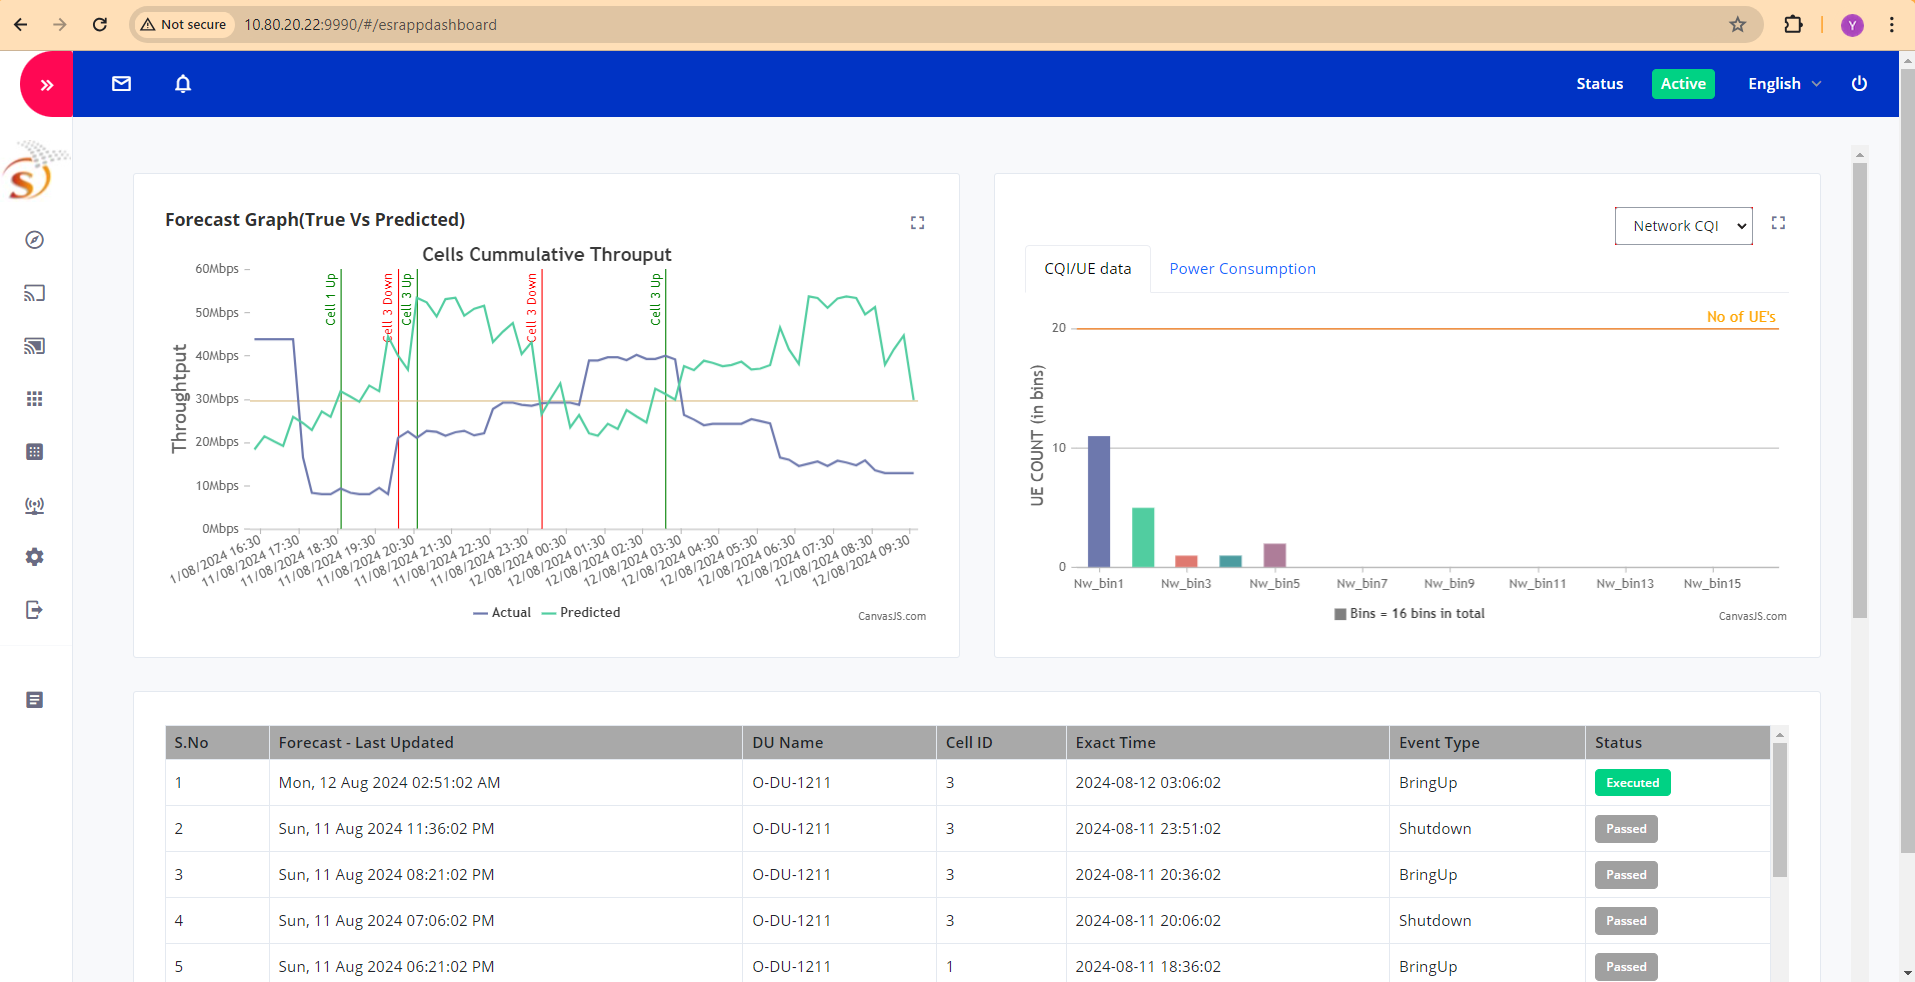
\includegraphics[width=0.5\textwidth]{/Users/pulakmehrotra/Desktop/SaankhyaLabs/es_oran_paper/acm_version_final/images/dashboard.png}
  \caption{ES rApp GUI}
  \label{fig:dashboard}
\end{figure}

\section{Design Rationale}
\label{sec:design_rationale}

In this section, we elucidate our reasoning behind the choice of regression model used to represent the overall network throughput.

\begin{comment}
\subsection{Decision Variables and Threshold Selection}

The decision-making process in any solution is governed by a set of decision variables that determine the course of action to be taken.
We proceed to evaluate the performance of our Energy Saving solution in terms of the three metrics mentioned below:
\begin{itemize}
  \item \textbf{Network CQI Distribution:} As described in [\textcolor{blue}{CITE}], we categorized the CQI values of the UEs based on the channel quality.
  \item \textbf{Network Throughput:} This metric represents the total throughput used by all the UEs connected to the system.
  \item \textbf{System Power Consumption:} This is the total power consumed by the system, measured in Watts (W).
\end{itemize}

The most important one to consider here is the throughput of the network, which is the primary metric used to decide whether a system needs a change in it's configiration or not.
The rationale behind this is simple: our focus is on the aggregate network performance, and throughput serves as a reliable metric for this purpose.
If the network state, specifically the channel quality and overall throughput, remains largely unchanged after the application of network-modifying policies, we deem the result acceptable.

The determination of thresholds for various decision variables is often crucial to the success of the algorithm. 
In this context, we aim to derive specific expressions to guide the selection of these variables.
In our proposed solutions, we have three primary decision variables: $\tau$, $\alpha_{th}$, and $P_{th}$.
- $\tau$ is the threshhold on the forecasted throughput, which is used to decide whether to shut down a cell or not.
- $\alpha_{th}$ is the allowed divergence of the forecasted/likely CQI distribution from the current CQI distribution. It is used to decide whether a policy should be implemented or not.
- $P_{th}$ is the threshold on the power consumption of the cell. Only cells function above a certain energy-consumption threshold are to be considered for shutdown/bringup.
\\
\textcolor{red}{[PRAMIT] \\
Could you please provide a short write-up on how $\tau$, $\alpha_{th}$ and $P_{th}$ are selected? What are the factors we consider?}
\end{comment}

\subsection{Datasets In Use}

We intended to find a regression model that, above all, identified the trend and seasonlity of traffic fluctuations.
The models underwent evaluation using a mix of four real-world and five synthetic time-series datasets, each exhibiting diverse trends and seasonal patterns:

\begin{itemize}
  \item Dataset 1: COMED Dataset - This real-world dataset, released by the Commonwealth Edison Company, illustrates the temporal variations in power consumption across a specific group of households.
  \item Dataset 2: Microsoft Dataset - This dataset, obtained using a data scraper, encapsulates the temporal variations in Microsoft's stock price.
  \item Dataset 3: Temperature Dataset - This dataset, sourced from Kaggle, depicts the temporal progression of the Earth's surface temperature.
  \item Dataset 4: No Trend Dataset - This synthetic dataset, created using a blend of sinusoidal and random noise functions, exhibits no discernible trend or seasonality.
  \item Dataset 5: Upwards Trend Dataset - This synthetic dataset is similar to Dataset 4, but it exhibits a noticeable upward trend (without any seasonality).
  \item Dataset 6: Downwards Trend Dataset - This synthetic dataset is similar to Dataset 4, but it exhibits a noticeable downward trend (without any seasonality).
  \item Dataset 7: Upwards Trend Dataset with Seasonality - Dataset 5 with added seasonality.
  \item Dataset 8: Downwards Trend Dataset with Seasonality - Dataset 6 with added seasonality.
  \item Dataset 9: Simulator Dataset - A synthetic dataset generated using our ns-3 simulator, taken to ensure that these models perform with traffic data and not just randomized time-serieses.
\end{itemize}

\subsection{Model Selection}
\begin{table*}[ht]
\caption{Performance of Different Models on Various Synthetic Datasets}
\centering
\resizebox{\textwidth}{!}{%
    \begin{tabular}{|*{3}{>{\centering\arraybackslash}p{0.33\textwidth}|}}
    \hline
    \textbf{Dataset Type} & \textbf{Prophet Performance} & \textbf{LSTM Performance} \\
    \hline
    No Trend, No Seasonality & Does not trend correctly, trends in the opposite direction & Follows trend but does not account for the noise well \\
    \hline
    Upwards Trend, No Seasonality & Steadily trends upwards but not according to the data (underfits) & Follows trend but predicts widely off values when accounting for noise \\
    \hline
    Downwards Trend, No Seasonality & Trends appropriately but underfits, does not recognize dataset intricacies & Recognizes trend and seasonality but produces very inaccurate values due to noise \\
    \hline
    Upwards Trend, With Seasonality & Recognizes trend but not seasonality & Recognizes trend and seasonality well, performs satisfactorily with test data \\
    \hline
    Downwards Trend, With Seasonality & Recognizes trend but not seasonality & Recognizes trend and seasonality but produces very inaccurate values due to noise \\
    \hline
    \end{tabular}%
}
\end{table*}

The choice of regression model used for Traffic Prediction is crucial to the success of the solution.
In this section, we compare the performance of three different regression models: Prophet, ARIMA, and LSTMs.
We train our models on all our real-world datasets (COMED, Microsoft and Temperature) and evaluate their performance on a validation set of the same dataset.
Our findings can be seen in \hyperref[tab:model_comp]{Table 1}.
We observe that the LSTM model outperforms Prophet, capturing the trend and seasonlity of the data the best.
The ARIMA model was found to be outright the worst performer, both taking the longest to train as well making forecasts completely ignoring the trend and seasonlity of the inputed data.
Considering how promising the LSTM's performance seemed, we decided to further evaluate the same.

\subsection{Model Verification}
\begin{table*}[ht]
    \caption{Performance of Different LSTM Models on Various Datasets}
    \centering
    \resizebox{\textwidth}{!}{%
      \begin{tabular}{|*{9}{>{\centering\arraybackslash}p{0.11\textwidth}|}}
        \hline
        \textbf{Dataset/Model} & \textbf{Model 1} & \textbf{Model 2} & \textbf{Model 3} & \textbf{Model 4} & \textbf{Model 5} & \textbf{Model 6} & \textbf{Model 7} & \textbf{Model 8} \\
        \hline
        \textbf{Model 1} & 0.044 & 0.0054 & 0.2507 & 2.0302 & 0.6256 & 1.8354 & 1.186 & 1.1158 \\
        \hline
        \textbf{Model 2} & 0.3358 & 0.2262 & 0.2609 & 0.915 & 0.2613 & 0.855 & 0.486 & 0.4774 \\
        \hline
        \textbf{Model 3} & 0.5695 & 0.7270 & 0.4274 & 1.0624 & 0.3611 & 1.091 & 0.6027 & 0.593 \\
        \hline
        \textbf{Model 4} & 1.0267 & 0.5424 & 0.7875 & 0.5457 & 0.7711 & 1.3335 & 0.6144 & 0.9841 \\
        \hline
        \textbf{Model 5} & 0.5713 & 0.6027 & 0.4731 & 1.069 & 0.2857 & 1.011 & 0.5556 & 0.5418 \\
        \hline
        \textbf{Model 6} & 1.3595 & 1.1141 & 1.3407 & 1.2204 & 0.9841 & 1.2831 & 1.0261 & 1.0280 \\
        \hline
        \textbf{Model 7} & 0.5459 & 0.3503 & 0.2500 & 0.9837 & 0.2005 & 0.9108 & 0.4610 & 0.4590 \\
        \hline
        \textbf{Model 8} & 0.5806 & 0.2504 & 0.1865 & 0.9605 & 0.1640 & 0.8965 & 0.417 & 0.4134 \\
        \hline
      \end{tabular}%
    }
  \end{table*}
  
  

After arriving at using LSTMs as the model of choice for traffic forecasting, we had to ensure that the model would be able to handle the simulated load. 
We did so using synthetic data of various types, as outlined in our Dataset section.
To verify the robustness of the model's forecasts, we trained the LSTM models using a diverse range of datasets, each exhibiting unique general trends.
For each dataset, we trained a corresponding LSTM model. 
We used Mean Squared Error (MSE) as an evaluation index to evaluate the forecast accuracy of the models.
Subsequently, we cross-validated each trained model with the remaining datasets.
The MSE values of all the trained models and the datasets in use is described in in \hyperref[tab:lstm_performance]{Table 2}.
We observe that the LSTM trained on data with more seasonlity (model 7,8 and 9) perform the best all around, with the lowest MSE values.
This is expected, as the LSTM model is designed to capture the long-term dependencies in the data, which are more prevalent in datasets with seasonality.
  
Therefore, when training our model on real-world data, we should ensure that the data has a significant amount of seasonality to ensure the best performance.  
The amount of data used to train the LSTM model is crucial to the success of the solution.
If we train the model on excessive data, the model may overfit to the training data and fail to generalize to unseen data.
This would be especially catastrophic in our specific use case, as we
This will depend on the deployemnt environment's complexity, and in our specific setup we found 300 samples to suffice.



\end{document}